\section{Machine Control}

\subsection{democratization of machines}

We should have as much control as possible of every machine we interact with and every machine which affects our lives and the lives of our communities.  We currently live in a time where our ability to control our own machines is decreasing very rapidly, and it is the intent of this work to build technology which reverses this trend. For the last few hundred years, as machines have become more powerful and complex there has been a constant conflict between machines' ability to reduce labor and their ability to also increase the power and control of whoever controls the machines.  In the early days of the Industrial Revolution we started to see battle lines being drawn around the forces of mechanization which rage as hot today as they did then.

The basic conflict of the Industrial Revolution was between laborers who saw machines as replacing their role in society and those who saw the machines as having an overall benefit to society at large by producing more products faster and more efficiently.  This conflict stemmed from the way we have structured labor and work during the time and place that these technologies came to power, namely the wage labor system.  Under wage labor, the more ``labor'' someone does, the more money they get to survive.  This creates an incentive for automation for the capitalist class, and create the opposite incentive in the laboring classes.  Marxists took this structure for granted and argued that the laboring classes could liberate themselves through political control, but took the basic premise of ``work'' or ``labor'' for granted as ideas.  

The time we find ourselves in today differs so vastly from that of the industrial revolution that we must pause and re-evaluate some assumptions.  The most fundamental assumption of the time of the Industrial Revolution which we must dispose of is the need for a constant stream of mined materials and materials extracted from far away places.  This element of industrial production is often hidden from the consumer but is far more fundamental than people often recognize.  Every early industrialization process, involved some type of empire-building over large land masses in order to build stable supply chains to maintain a flow of materials from mine to factory to consumer.  The more deeply one studies industrialization the more clear this becomes. Some countries industrialized without building their own empires, but they did so by leveraging powerful trade relationships with existing empires.  In all cases, the power of the physical network of raw materials was what made or broke the process. 

But today the world we live in it materially different in this fundamental way: all the materials of a mechanized civilization are now readily available everywhere in the world, without exception.  The global consumer industrial capitalist system has consumed the mineral wealth of the last 300 years of imperialism and industrialization remarkably evenly through the world by pushing the same consumer products everywhere, all of which form localized waste streams of highly processed materials.  

Just take aluminum as one example.  Aluminum is one of the most powerful tools we have ever discovered to create technology, with a very wide range of uses.  However, before we can even shape it we have to reduce the bauxite ore, which is a very energy intensive process. I strongly recommend that the reader spend some time choosing random elements like aluminum or phosphate and learning where they come from.  All the minerals we use take vast amounts of energy and complex mechanical processes.  And yet, all of them are now free!  If we want to use aluminum in a technology today not only do we not have to reduce the ore to pure metal, we don't even have to machine it.  We can find fully processed and coated aluminum shaped into already-useful shapes from beer cans to light poles.  If we build our civilization on this waste stream, all the assumptions of politics and economics from the last 300 years of Western thought must be abandoned.  

Today, we can build machines directly from the materials we find in our environment, without the need for a global supply chain we control.  Even if the existing supply chains collapse, the existing cache of waste we find in our immediate environment should be sufficient to live technologically advanced lives.  Therefore, under these new material conditions, machine control is direct, physical, and built into the design of the machine, rather than based on ``power'' in relation to large organizations like nation-states and corporations.  

[all the above paragraphs should move to chapter 1, then just get referenced here as we dive into the following list of principles]

If our goal is to have the most control possible over our own lives in a technological society, we now aim to design that control directly into the machines. Democratization of this control(avoiding building a power elite of technology experts) then becomes a task of user interface design.  If we look at the last few hundred years of building labor-saving machines, we find some good things and some bad things.  In this work, I aim to create a framework for making those choices and for building technology which follows the principle that the more direct control the individual has over their technology the better, and will now delineate those principles.  

\textbf{Direct control before automation.}  This means every operation of a machine has a physical control which a user can use to directly control that operation.  If a tool can be moved up, down, left, right, forward, and back, we will always have a controller which enables them to directly carry out that action without any further automation.  This controller should be as physical as possible(rather than through software and touch screens).  Unlike the automation discussed below, it will generally be as continuous as possible, allowing a user to directly move small or large distances with feedback being directly trough observation of the machine outside of any control technology.

\textbf{Controllers are sized for humans.}  We want controllers which are as closely matched to how humans think, feel, and act as possible.  This means things will be much bigger and more redundant than they need to be by the absolute minimal requirements of control.  Buttons and levers will be as large as they have to to allow the absolute maximum range of human users to operate it without difficulty.  We will not have defaults be small buttons and have a special case with large buttons, but will always have buttons sized for people with limited sight or dexterity.  

\textbf{Controls should use geometry to be obvious.}  A lever next to a hoist should have pulling it up move the hoist up, and down be down.  A pair of buttons should have the top one move up and bottom one move down.  We also shape the controls to have geometric meaning as much as possible, for instance shaping a button as a physical arrow pointing in the direction of the motion it causes.  

\textbf{All actions should be convertible to automation.}  This means if we can use a controller to move a tool along some path, we can build a program which repeats that action with a single button press.  Thus a controller will have, in addition to the direct controls, a ``go'' button which will initiate the automation program.  The previous two principles dictate that this button be large, green, and round.

\textbf{All automation actions can be stopped at any time.}  The big red ``stop'' button must also be universal. Pushing this button immediately stops the automating action.  This is different from the ``EPO'' or Emergency Power Off button which can also be a good idea, which shuts down a machine completely.  A stop button simply stops whatever action was initiated by the go button.

\textbf{Discrete geometric actions of Geometron, using geometric symbols enable programming with no specialized technical knowledge.}  This is the heart of where Geometron enables 

\textbf{Symbol hierarchy.}  Symbols are used describe action sequences which are built up to make more complex actions.  

\textbf{Upcycled hardware.}  This is the principle used throughout this work, but must be re-emphasized here because it is so important and because it is so easy for controllers.  



\begin{itemize}
\tightlist
\item
introduction, the democratization of automation
\item
structure of hypercube, workflow, general principles
\item
trash robot printer
\item
wall robot on large building
\item
agricultural robot prototype/description
\item
electron beam lithography
\item
hacked 3d printer to make 2.5d printer
\end{itemize}


\begin{figure}
	\centering
	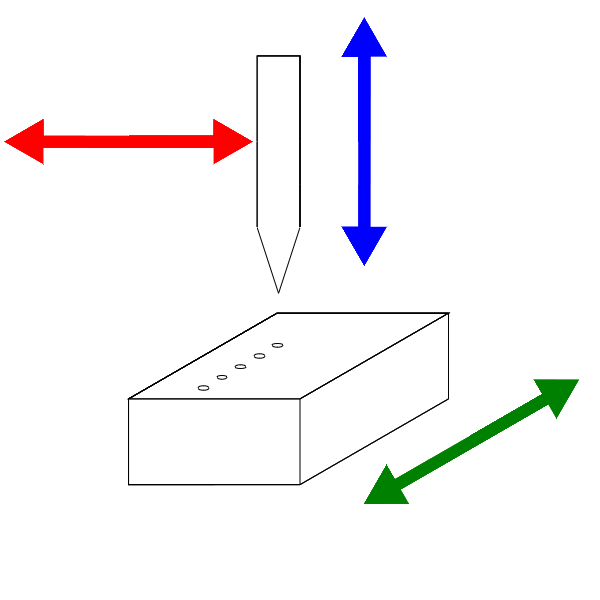
\includegraphics[width=4in]{figures/machines/xyzprobe.png}
	\caption[xyzprobe]
	{A probe move over a sample in either the x or z direction, and the sample moves along the y axis.  Repeated poking of the sample prints dots a simple but very versatile tool.}
\end{figure}


\begin{figure}
	\centering
	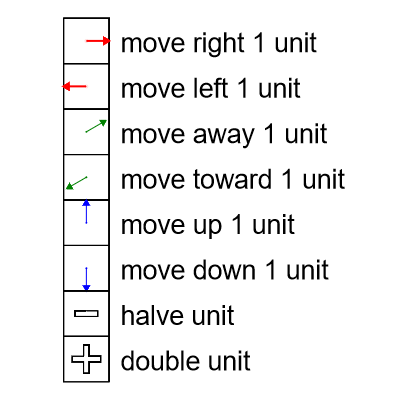
\includegraphics[width=4in]{figures/machines/basicmovements.png}
	\caption[basicmovements]
	{Basic geometric actions of machine control for an arbitrary machine that moves along three perpendicular axes.}
\end{figure}

\begin{figure}
	\centering
	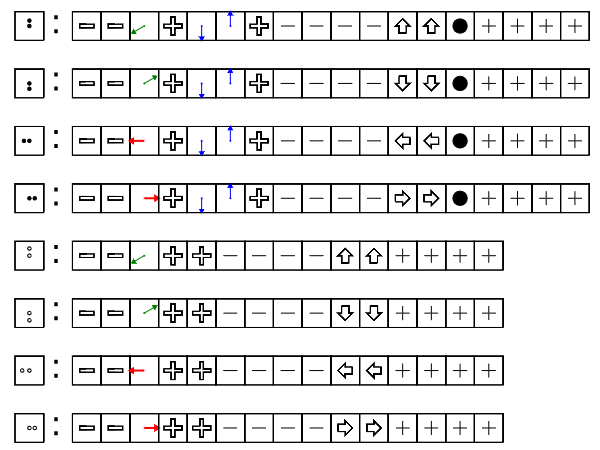
\includegraphics[width=4in]{figures/machines/actions05xx.png}
	\caption[actions05xx]
	{Dot actions from which symbols are constructed.}
\end{figure}


\begin{figure}
	\centering
	
\includegraphics[width=4in]{figures/machines/buildingwallrobot.png}
	\caption[buildingwallrobot]
	{A hoist run along a rail going across the edge of a roof of a building can make a simple robot which can move to anywhere along the wall.}
\end{figure}
